\documentclass[a4paper,11pt]{report}

\usepackage[T1]{fontenc}
\usepackage[utf8]{inputenc}
\usepackage[italian]{babel}

\usepackage{wrapfig}
\usepackage{mathtools}
\usepackage{graphicx}
\usepackage{amsfonts}
\usepackage{amsthm}
\usepackage{amsmath}
\usepackage{amssymb}
\usepackage{fancyhdr}
\usepackage{float}
\usepackage{geometry}
\geometry{a4paper, top=2.5cm, bottom=2cm, left=2cm, right=2cm}
\usepackage{hyperref}
\hypersetup{
	colorlinks=true,
	linkcolor=black,
	filecolor=blue,
	citecolor = black,      
	urlcolor=cyan,
}

\begin{document}
	\date{}
	\author{Marco Militello}
	\title{Chimica}
	\maketitle
	\tableofcontents
	\newpage
	
\chapter{Introduzione}
La chimica è lo studio della materia, delle sue proprietà, delle trasformazioni subite dalla materia e dell'energia associata a queste trasformazioni
\begin{description}
	\item[Materia] Tutto ciò che ha una massa e un volume
	\item[Composizione] I tipi e le quantità di sostanze più semplici che costituiscono la materia
	\item[Proprietà] Le caratteristiche che conferiscono a ciascuna sostanza la sua identità esclusiva 
\end{description}
\section{Stati aggregazione della materia}
\begin{itemize}
	\item Un \emph{solido} ha forma e volumi fissi. I solidi possono essere duri, teneri, rigidi o flessibili
	\item Un \emph{liquido} si adatta alla forma del recipiente, ma un volume fisso. Un liquido forma una superficie
	\item Un \emph{gas} si adatta alla forma del recipiente e lo riempie completamente, perciò non forma una superficie
\end{itemize}
\section{Proprietà della materia}
\subsection*{Proprietà fisiche}
Le proprietà che una sostanza presenta di per sè senza trasformasi in, o interagire con, un'altra sostanza
\begin{itemize}
	\item[-] colore, temperatura di fusione, densità
\end{itemize}
\subsection*{Proprietà chimiche} 
Le proprietà che una sostanza presenta quando si trasforma in, o interagisce con, un'alra sostanza
\begin{itemize}
	\item[-] infiammabilità, corrosività
\end{itemize}
\section{Composizione della materia}
\subsection*{Sostanze pure}
Una sostanza che ha proprietà e composizione proprie, che non dipendono dal campione \newline
Le sostanze pure possono essere sostanze elementari (\emph{elementi}) o \emph{composti}. I composti possono essere trasformati in sostanze elementari tramite trasformazioni chimiche
\subsection*{Miscele}
Una sostanza che ha una composizione variabile, le cui proprietà dipendono dal campione analizzato \newline
Le miscele possono essere separate nelle sostanze costituenti mediante metodi fisici
\begin{figure}[H]
	\centering
	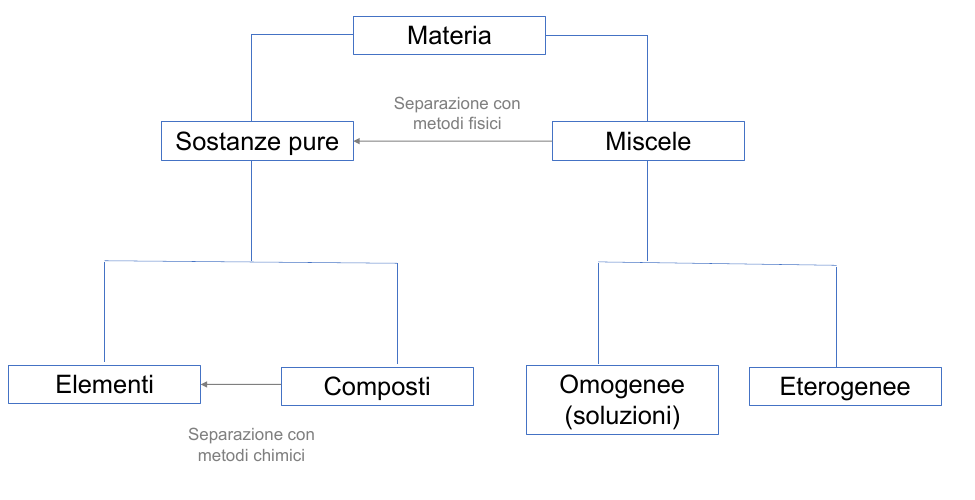
\includegraphics[width=\textwidth,height=\textheight,keepaspectratio]{immagini/grafico1}
	\label{fig:grafico1}
\end{figure}
\chapter{Teoria atomica}
\section{Teoria atomica di Dalton}
\begin{enumerate}
	\item Tutta la materia è costituita da atomi, piccole particelle indivisibili di un elemento che non possono essere nè create, nè distrutte
	\item Gli atomi di un elemento non possono essere convertiti in atomi di un altro elemento
	\item Gli atomi di un elemento sono identici nella massa e nelle altre proprietà e sono diversi dagli atomi di qualsiasi altro elemento \label{3}
	\item I composti sono formati dalla combinazione di uno specifico rapporto di atomi differenti
\end{enumerate}
\noindent La teoria di Dalton spiega le leggi delle combinazioni chimiche
\begin{itemize}
	\item Legge della composizione definita \hfil\\
	Indipendentemente dalla sua fonte, un particolare composto chimico è costituito dagli stessi elementi negli stessi rapporti in massa
	\item Legge della conservazione della massa \hfill\\
	In base al postulato \hyperref[3]{3} della legge di Dalton gli atomi, e quindi la loro massa, vengono conservati nelle reazioni chimiche
\end{itemize}
\section*{Scoperta delle particelle sub-atomiche: raggi catodici}
\begin{itemize}
	\item Il raggio devia in presenza di un campo elettrico o magnetico $\Rightarrow$ Consiste in particelle cariche di cui si determina il rapporto carica/massa
	\item In presenza di un campo elettrico esterno il raggio devia verso la rica positiva $\Rightarrow$ Consiste in particelle negative
	\item Il raggio è identico per ogni catodo $\Rightarrow$ Le particelle fanno parte di tutta la materia
\end{itemize}
\subsection*{Esperimento di Millikan}
\begin{figure}[H]
	\centering
	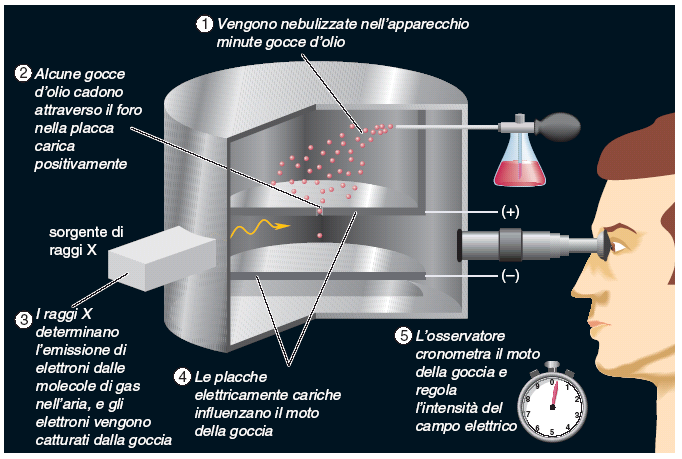
\includegraphics[width=0.5\textwidth,height=\textheight,keepaspectratio]{immagini/Millikan}
	\label{fig:millikan}
\end{figure}
\[\text{massa elettrone} = \left(\frac{massa}{carica}\right)carica = 9.109 \times 10^{-28}g  \]
\begin{figure}[H]
	\centering
	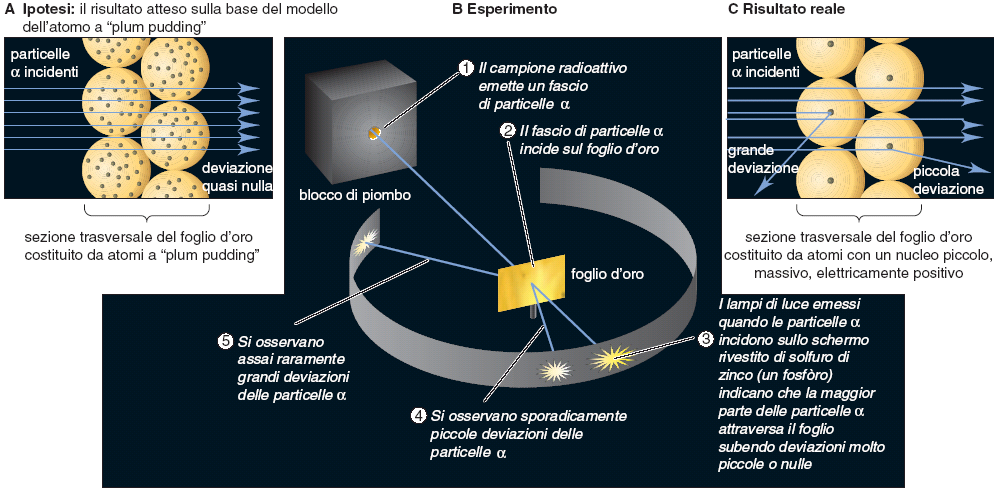
\includegraphics[width=\textwidth,height=\textheight,keepaspectratio]{immagini/atomo}
	\caption{}
	\label{fig:atomo}
\end{figure}
\begin{figure}[H]
	\centering
	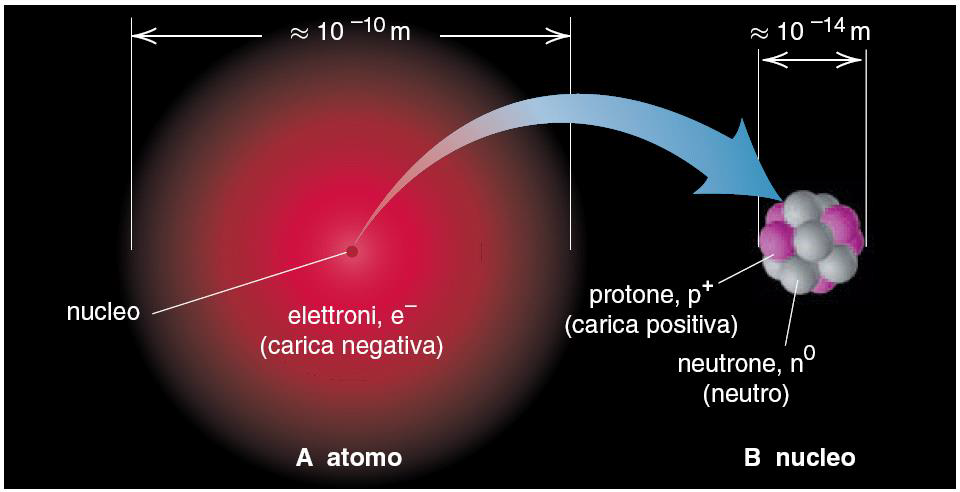
\includegraphics[width=0.5\linewidth, height=\textheight,keepaspectratio]{immagini/atomo1}
	\label{fig:atomo1}
\end{figure}
\begin{itemize}
	\item [A.] Una nuvola di elettroni carichi negativamente, in modo rapido, occupa pressochè tutto il volume atomico e circonda il minuscolo nucleo centrale
	\item [B.] Il nucleo contiene pressochè tutta la massa dell'atomo ed è costituito da protoni carichi positivamente e neutroni elettricamente neutri
\end{itemize}

\section{Simbolo atomico, numero atomico e numero di massa}

\begin{figure}[H]
	\centering
	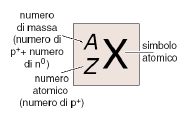
\includegraphics[width=0.2\linewidth, height=\textheight,keepaspectratio]{immagini/numero.png}
	\label{fig:numero}
\end{figure}

\begin{center}
\begin{tabular}{|c|c|}
	\hline
	X & simbolo atomico dell'elemento \\
	\hline
	Z & numero atomico (numero di protoni nel nucleo) \\
	\hline
	A & numero di massa	\\
	\hline
\end{tabular}
\end{center}

\[A = Z+N\]

\subsection*{Isotopi}

Gli isotopi sono atomi di un elemento con lo stesso numero di protoni, ma con diverso numero di neutroni; gli isotopi hanno lo stesso numero atomico, ma diverso numero di massa

\subsection*{Teoria atomica moderna}

\begin{enumerate}
	\item Tualla la materia è costituita da atomi. L'atomo è la particella più piccola che identifica univocamente un elemento 
 \item Gli atomi di un elemento non possono trasformarsi negli atomi di un altro elemento in una trasformazione chimica. Elementi possono convertiti in atri elementi solo in una reazione nucleare 
 \item Tutti gli atomi di un elemento hanno lo stesso numero di protoni e elettroni che determina il comportamento chimico dell'elemento. Gli isotopi di un elemento differiscono nel numero di neutroni, dunque nel numero di massa. Un campione di elemento viene considerato come se tutti i suoi atomi avessero una massa mediante
 \item i composti sono formati dalla combinazione chimica di due o più elementi in rapporti specifici
\end{enumerate}

\subsection*{Tecniche di separazione fondamentali}

\begin{description}
	\item[Filtrazione:] separa i componenti di una miscela sulla base di differenze tra le dimensioni delle particelle. La filtrazione viene usata spesso per separare un solido da un liquido 
 \item[Cristallizzazione:] la separazione è basata sulle differenze di solubilità dei componenti di una miscela 
 \item[Distillazione:] separa i componenti sulla base di differenze di volubilità 
 \item[Estrazione:] la separazione è basata sulle differenze di solubilità in diversi solventi
 \item[Cromatografia:] la separazione è basata sulle differenze di solubilità in una fase stazionaria     
\end{description}


\end{document}